\section{Programmable timers}

A programmable timer is a specialized clock used to measure time intervals or count events, and it is a fundamental component in many embedded systems. 
Timers can operate in different modes, either counting upwards to measure elapsed time (like a stopwatch) or counting downwards to generate a delay for timing purposes. 
Additionally, timers often incorporate counters, which track and record the number of events triggered by external signals.
\begin{figure}[H]
    \centering
    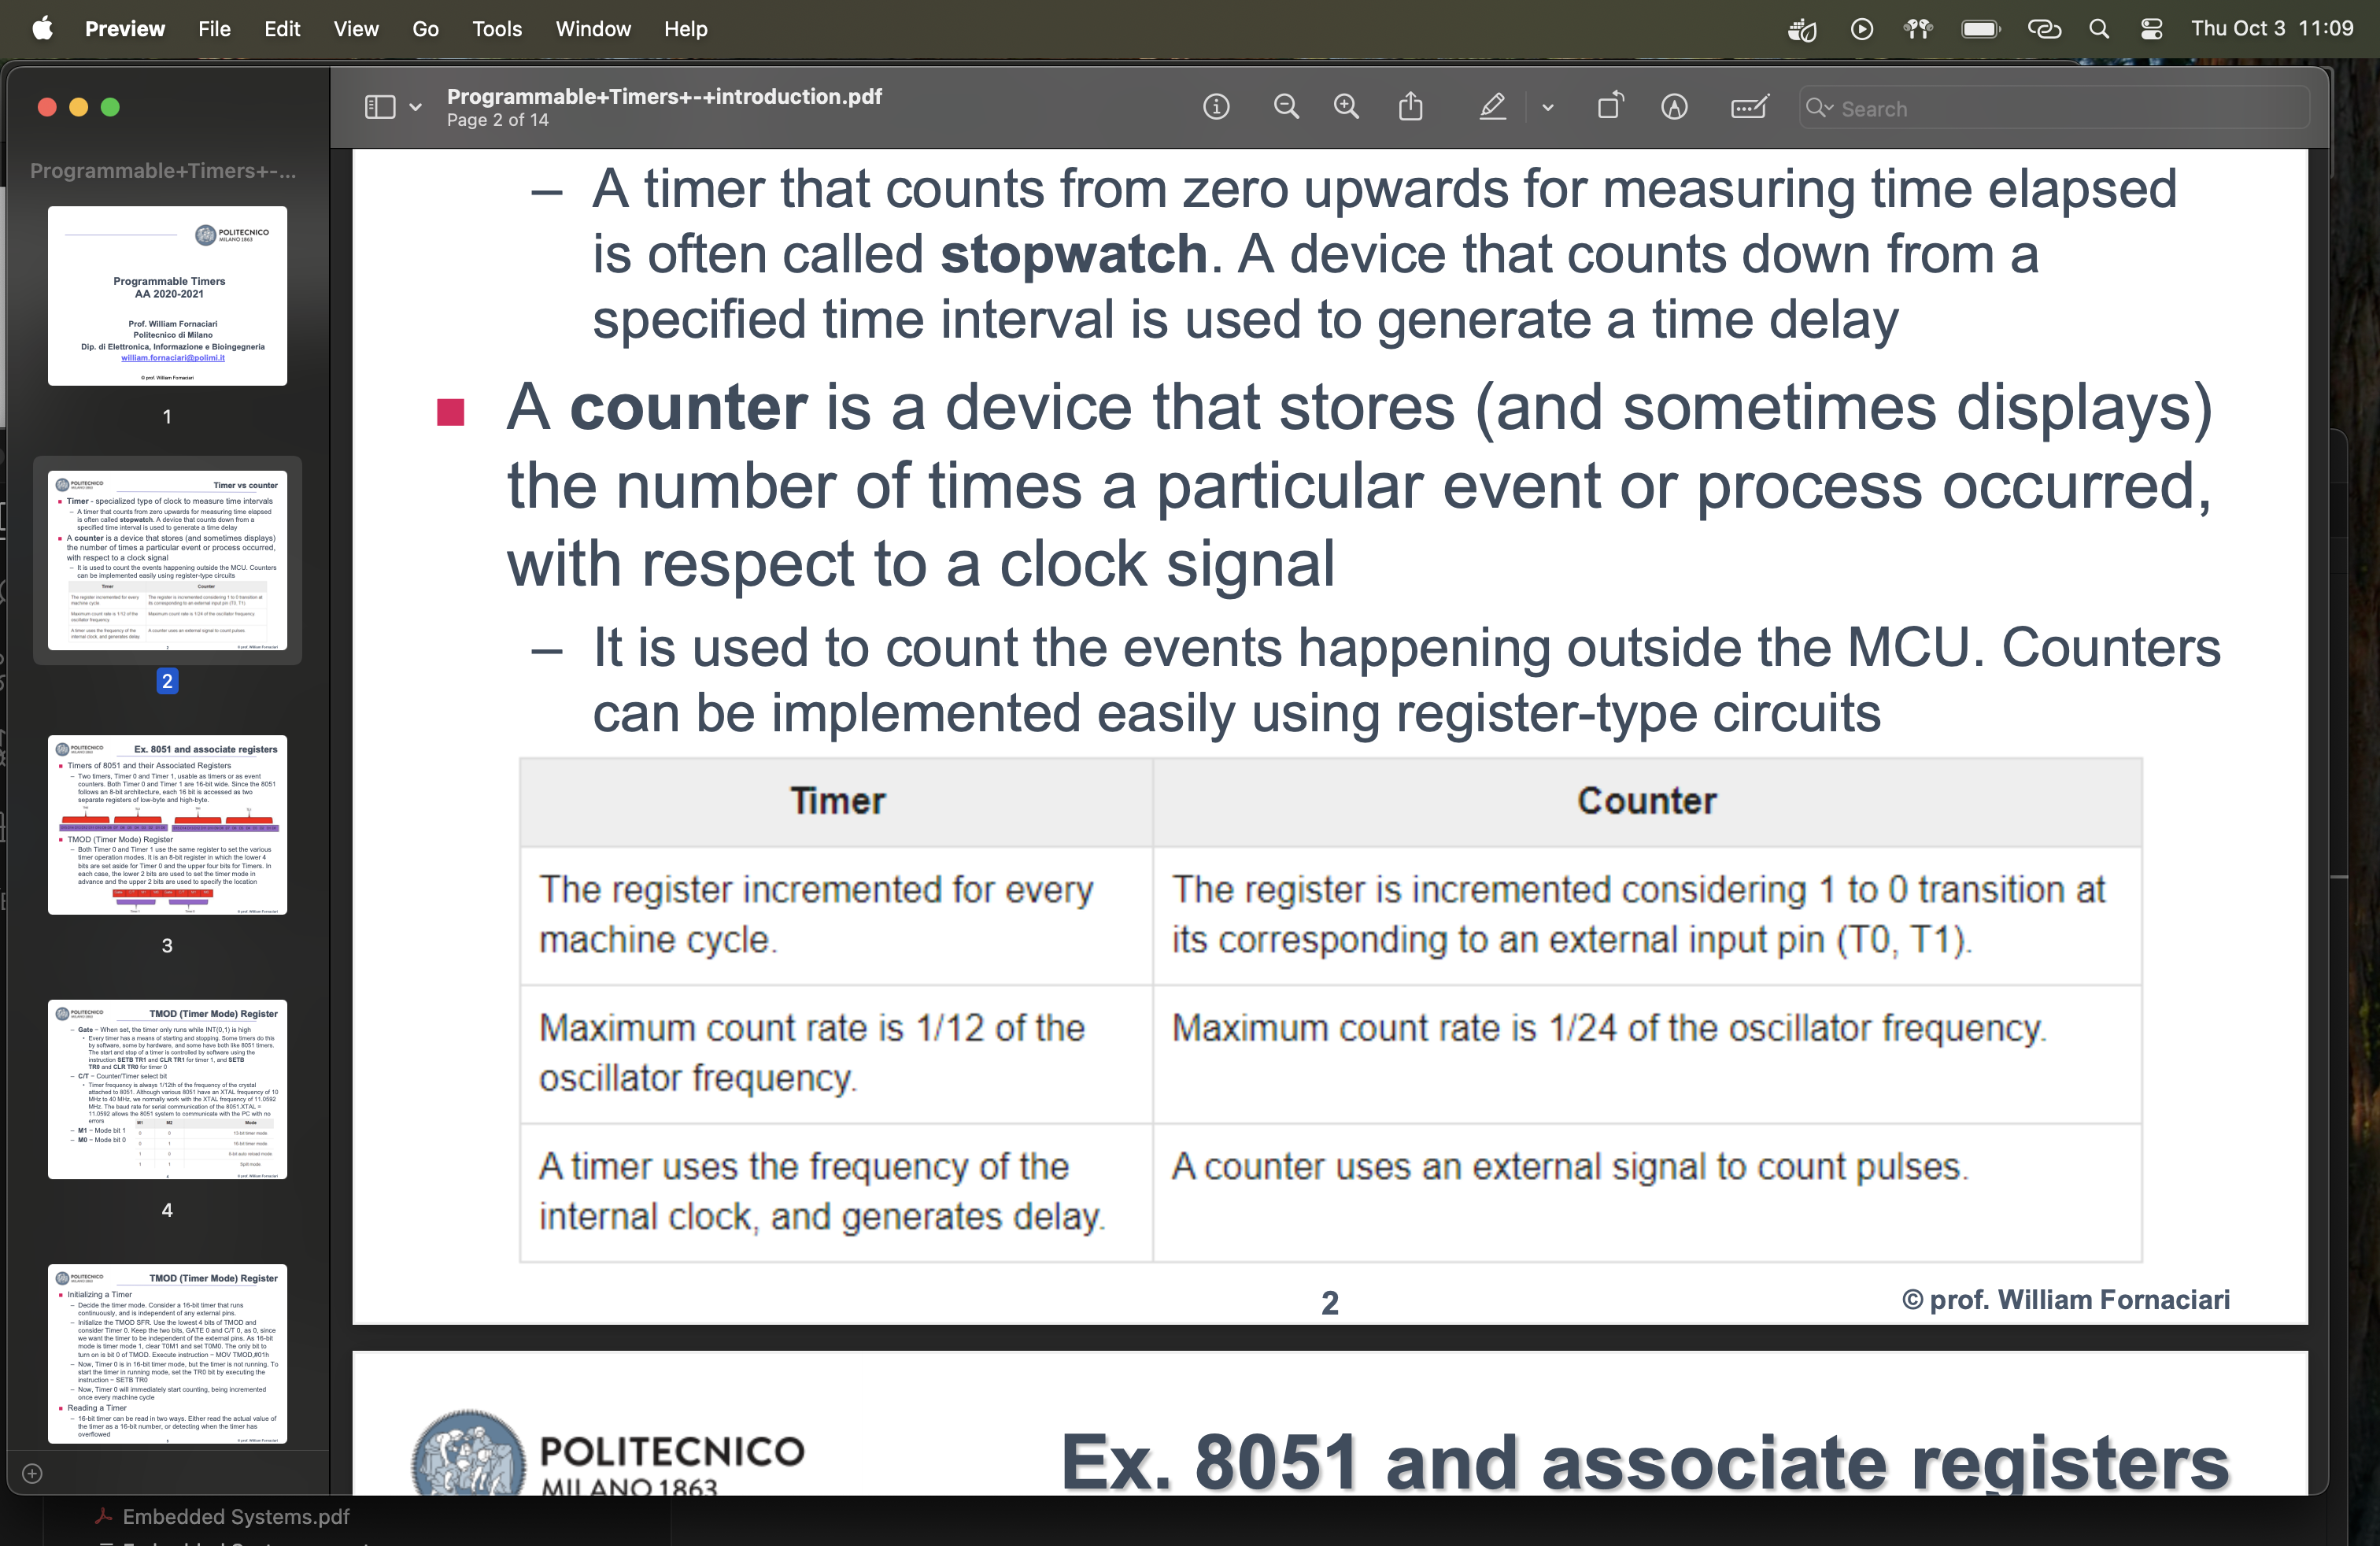
\includegraphics[width=0.75\linewidth]{images/tim.png}
\end{figure}

\paragraph*{Counters}
Counters are similar to timers but are designed to count external events (e.g., signal pulses) instead of clock cycles. 
They are useful in tracking occurrences of specific events such as input signals, sensor triggers, or external interrupts.

In microcontroller-based systems, timers and counters are widely used for generating time delays, event counting, and more. 
Counters are implemented using register-based circuits, which can store and display the number of events or clock cycles that have occurred.

\subsection{Operations and settings}
\paragraph*{Timer Mode registers}
Timers are controlled through Special Function Registers (SFRs) that define how the timer operates. 
The configuration options typically include:
\begin{itemize}
    \item \textit{Gate}: when set, the timer only runs while an external interrupt is active (high). 
        Otherwise, the timer operates continuously.
    \item \textit{Start and stop control}: timers can be started and stopped via software or hardware control. 
    \item \textit{Counter or timer select bit} (C/T): this bit determines whether the module operates as a timer (incrementing with the internal clock) or a counter (incrementing based on external events). 
\end{itemize}

\paragraph*{Initialization}
To initialize a timer, the configuration process typically involves setting the appropriate bits in the timer's control register. 
Below is an example for initializing a 16-bit timer that operates continuously without external pin dependencies:
\begin{enumerate}
    \item Select timer mode: we will configure Timer 0 to operate in 16-bit mode, which allows the timer to count from 0 to 65535 before overflowing.
    \item Initialize the TMOD register: set the timer mode by modifying the lower 4 bits of the TMOD register. 
    \item Execute the instruction \texttt{MOV TMOD, \#01h} to configure Timer 0.
    \item Start the Timer: after configuring the timer, start it by setting the \texttt{TR0} bit, which starts the timer incrementing with every machine cycle.
        Execute \texttt{SETB TR0} to start Timer 0.
\end{enumerate}
Now, Timer 0 will begin counting, incrementing once every machine cycle, and will continue until it overflows or is manually stopped.

\paragraph*{Reading}
There are two primary ways to read the value of a 16-bit timer:
\begin{itemize}
    \item \textit{Reading the timer value}: you can read the actual count value stored in the timer registers. 
        This provides the current count, allowing you to measure elapsed time or events.
    \item \textit{Detecting timer overflow}: alternatively, you can monitor the timer overflow flag, which is set when the timer reaches its maximum value (e.g., 65535 in a 16-bit timer). 
        Once overflow occurs, the timer resets and starts counting from zero again.
        This is useful for generating interrupts or periodic signals.
\end{itemize}
By configuring the timer to trigger an interrupt on overflow, you can create precise, repeatable time delays or event-driven processes in your system.

\paragraph*{Settings}
Timers can be operated either by polling or by using interrupts:
\begin{itemize}
    \item \textit{Polling}: this involves continuously reading the status registers to check for timer events or the current counter value. 
        However, polling can consume significant processing time and may introduce variability in response times, especially in complex programs.
    \item \textit{Interrupts}: a more efficient approach is to configure the timer to generate an interrupt when a specific event occurs. 
        When the event occurs, the timer triggers a hardware signal that is sent to the microcontroller's interrupt controller, which suspends the main program and jumps to an Interrupt Service Routine (ISR).
        After executing the ISR, the program returns to its main loop. 
        This method ensures fast and predictable responses to timer events, without requiring the main program to check for them continuously.
\end{itemize}

\subsection{Structure}
The basic structure of a timer in an microcontroller consists of several essential components:
\begin{itemize}
    \item Clock source: every timer requires a clock to measure time intervals. 
        Multiple clock sources may be available, with the possibility of selecting an external clock if needed.
    \item Prescaler: to extend the count range, the clock signal is passed through a prescaler, which divides the input clock by a factor (often a power of 2). 
        Some prescalers allow division by factors as large as $2^{16}$ (up to 65536).
    \item Main counter: after the prescaler, the clock feeds into a main counter. 
        Typically 16 bits wide, this counter can count up to 65,535. 
        It increments or decrements depending on the timer mode.
    \item Modulus Value (M): the main counter's range is controlled by a modulus value, which can be programmed into a register.
        When the counter reaches zero, it reloads this value and continues counting. 
        This configuration allows for generating periodic signals or interrupts.
    \item Control logic: the control logic defines the operational mode of the timer. 
        This includes configuring the clock source, prescaler, modulus value, and other control bits. 
        The control registers vary across different microcontrollers, providing flexibility to adapt the timer to different applications.
\end{itemize}
Typical initial configurations for an microcontroller timer include:
\begin{itemize}
    \item Selecting the appropriate clock source.
    \item Setting a prescaler value.
    \item Programming the modulus value.
    \item Configuring control bits to define the timer mode.
    \item Enabling interrupts (if required).
    \item Setting up peripheral triggers, such as Direct Memory Access (DMA) or other microcontroller peripherals.
    \item Configuring input/output pin connections if the timer is used for signal generation or external event detection.
\end{itemize}

\subsection{Periodic timers}
Periodic timers are used to generate repetitive events or ticks with a fixed period. 
The key parameter in such applications is the period, which is determined by the modulus value programmed into the timer. 
Periodic timers are commonly used for:
\begin{itemize}
    \item Generating the baud rate clock for serial communication.
    \item Polling digital inputs, such as pushbuttons, at regular intervals.
    \item Scheduling tasks in real-time operating systems (RTOS) based on precise time intervals.
    \item Pacing DMA transfers to peripherals such as Digital-to-Analog Converters (DACs).
    \item Triggering Analog-to-Digital Converters (ADCs) to ensure accurate sample rates.
\end{itemize}
Periodic timers provide a highly reliable mechanism for scheduling and synchronization in embedded systems, ensuring that events occur at precisely controlled intervals.

\subsection{Delay functions}
Delay timers are used to execute actions after a specific time interval has passed. 
This function works by resetting the timer to zero (event A) and waiting for a defined number of ticks before triggering the desired action (event B).
Delays are essential for:
\begin{itemize}
    \item Implementing debounce mechanisms for pushbuttons.
    \item Waiting for peripherals to complete their operations.
    \item Introducing pauses in the operation of mechanical systems or communication protocols.
\end{itemize}
By using programmable timers in microcontroller design, developers can achieve highly precise control over time-sensitive operations, ensuring that embedded systems can meet real-time constraints and efficiently manage resources.

\subsection{Microcontrollers design}
Timers and counters are some of the most critical peripherals in microcontroller designs, enabling a wide variety of functions that improve performance, reduce power consumption, and simplify designs. 
They can offload repetitive tasks from the CPU by handling timing-based operations through interrupts, freeing the processor to focus on more complex tasks.
\begin{itemize}
    \item Timers and counters can be used in virtually any application to enhance performance, reduce power usage, or streamline design by replacing CPU-based operations with interrupt-driven tasks.
    \item Many Commercial Off-The-Shelf (COTS) microcontroller devices include built-in support for programmable timers, enabling easy integration into designs.
    \item Some of the most sophisticated uses of timers are in Pulse Width Modulation (PWM) applications, such as motor control. 
        Here, hardware handles most of the PWM functions, minimizing processor involvement in low-level operations.
    \item Manufacturers provide development kits and reference designs tailored to specific applications that rely heavily on programmable timers.
\end{itemize}